\documentclass[draft]{ametsoc}
\usepackage{color}
\usepackage{hyperref}
\journal{jhm}
%  Please choose a journal abbreviation to use above from the following list:
%
%   jamc     (Journal of Applied Meteorology and Climatology)
%   jtech     (Journal of Atmospheric and Oceanic Technology)
%   jhm      (Journal of Hydrometeorology)
%   jpo     (Journal of Physical Oceanography)
%   jas      (Journal of Atmospheric Sciences)
%   jcli      (Journal of Climate)
%   mwr      (Monthly Weather Review)
%   wcas      (Weather, Climate, and Society)
%   waf       (Weather and Forecasting)
%   bams (Bulletin of the American Meteorological Society)
%   ei    (Earth Interactions)

%%%%%%%%%%%%%%%%%%%%%%%%%%%%%%%%
%Citations should be of the form ``author year''  not ``author, year''
\bibpunct{(}{)}{;}{a}{}{,}
\title{Title here}

\authors{Andrew N. Other
and Fred T. Secondauthor
\thanks{Current address: Some other place, Germany}
}
\affiliation{American Meteorological Society,Boston, Massachusetts}


\extraauthor{Ping Lu
\correspondingauthor{Ping Lu,American Meteorological Society, 45 Beacon St., Boston, MA 02108.}
}
\extraaffil{Princeton University}
\email{groupleader@unknown.uu}
\extraauthor{Miao Yu
\thanks{Current address: Some other place, Canada}
}
\extraaffil{University of Waterloo}

% Pandoc citation processing

% pandoc header
\abstract{Enter the text of your abstract here. This is a sample American
Meteorological Society (AMS) \LaTeX~template. This document provides
authors with instructions on the use of the AMS \LaTeX~template. Authors
should refer to the file amspaper.tex to review the actual \LaTeX~code
used to create this document. The template.tex file should be modified
by authors for their own manuscript.}
\begin{document}
\maketitle
\hypertarget{introduction}{%
\section{Introduction}\label{introduction}}

This document will provide authors with the basic American
Meteorological Society (AMS) formatting guidelines. This document was
created using \LaTeX~and demonstrates how to use the \LaTeX~template
when submitting a manuscript to the AMS. The following sections will
outline the guidelines and formatting for text, math, figures, and
tables while using \LaTeX/ for a submission to the AMS. An attempt to
compile amspaper.tex should be made before using the template. The files
have been tested on Windows, Linux, and Mac OS using \TeX~Live 2011
(available online at \url{http://www.tug.org/texlive/}). Feedback and
questions should be sent to latex@ametsoc.org. Additional information is
available on the AMS \LaTeX~Submission Info web page
(\url{http://www2.ametsoc.org/ams/index.cfm/publications/authors/journal-and-bams-authors/author-resources/latex-author-info/}).

Authors should use the empty template.tex to begin their paper. A
valuable source of \LaTeX~information is the \{TeX Frequently Asked
Questions\} page (available online at \url{faq.tug.org}).

\hypertarget{formatting-text-and-sections}{%
\section{Formatting text and
sections}\label{formatting-text-and-sections}}

The text should be divided into sections, each with a separate heading
and consecutive numbering. Note, however, that single secondary,
tertiary, and quaternary sections remain unnumbered. Each section
heading should be placed on a separate line using the appropriate
\LaTeX~commands.

\hypertarget{secondary-headings}{%
\subsection*{Secondary headings}\label{secondary-headings}}
\addcontentsline{toc}{subsection}{Secondary headings}

Secondary headings labeled with letters are formatted using the
\texttt{\#\#\ Secondary\ headings\ \{-\}} for a single subsection within
a section or \texttt{\#\#\ Secondary\ headings} for multiple subsections
within one section.

\hypertarget{tertiary-headings}{%
\subsubsection*{Tertiary headings}\label{tertiary-headings}}
\addcontentsline{toc}{subsubsection}{Tertiary headings}

Tertiary headings are formatted using the
\texttt{\#\#\#\ Tertiary\ headings\ \{-\}} for single a subsubsection
within a subsection or \texttt{\#\#\#\ Tertiary\ headings} for multiple
subsubsections within a subsection.

\paragraph*{Quaternary headings}

Quaternary headings are formatted using the
\texttt{\textbackslash{}paragraph*\{Quaternary\ headings\}} for a single
paragraph within a subsubsection or
\texttt{\textbackslash{}paragraph\{Quaternary\ headings\}} for multiple
paragraphs within a subsection.

\hypertarget{citations}{%
\section{Citations}\label{citations}}

Citations to standard references in text should consist of the name of
the author and the year of publication, for example, Pöhlker et al.
(2012) or (Pöhlker et al. 2012; Alexander et al. 2002; Gershunov and
Guirguis 2012) using the appropriate \texttt{@key} or
\texttt{{[}@key{]}} commands, respectively. A variety of citation
formats can be used with the natbib package; however, the AMS prefers
that authors use only the \texttt{@key} and \texttt{{[}@key{]}}
commands. References should be entered in the references.bib file. For a
thorough discussion of how to enter references into the references.bib
database file following AMS style, please refer to the
\textbf{AMS\_Refs.pdf} document included in this package.

\hypertarget{formatting-math}{%
\section{Formatting math}\label{formatting-math}}

The following sections will outline the basic formatting rules for
mathematical symbols and units. In addition, a review of the
amspaper.tex file will show how this is done with the use of
\LaTeX~commands. The AMS template provides the American Mathematical
Society math, font, symbol, and boldface packages for use in math mode.

\hypertarget{mathematical-symbols}{%
\subsection{Mathematical symbols}\label{mathematical-symbols}}

Symbols must be of the same font style both in text discussion and in
displayed equations or terms (and figures should be prepared to match).
Scalar single-character symbols are set italic, Greek, or script.
Examples are \(u\), \(L\) {[}note that \(\upsilon\) (Greek upsilon) is
used instead of \emph{v} (italic ``vee'') to avoid confusion with
\(\nu\) (Greek nu) often used for viscosity; this is handled
automatically when in \LaTeX~math mode{]}, \(w\), \(x\), \(y\), \(z\),
\(f\), \(g\), \(r\), indices such as \(i\) or \(j\), and constants such
as \(C_D\), \(k\), or \(K\). Multiple-character scalar variables,
abbreviations, nondimensional numbers, and acronyms for variables are
set regular nonitalic: \(\mathrm{LWC}\), \(\mathrm{Re}\),
\(\mathrm{Ro}\), \(\mathrm{BT}\), \(\mathrm{abs}\), \(\mathrm{obs}\),
\(\mathrm{max}\), \(\mathrm{min}\), \(\mathrm{Re}\)/\(\mathrm{Im}\)
(real/imaginary), etc. For vectors, use boldface nonitalic Times Roman
as in \(\mathbf{V}\), \(\mathbf{v}\), or \(\mathbf{x}\), and
\(\mathbf{i}\), \(\mathbf{j}\), and \(\mathbf{k}\) unit vectors. Do not
use the \LaTeX~\(\backslash vec\) command to denote vectors. For matrix
notation, use nonitalic boldface Arial (or sans serif) font as in
\(\pmb{\mathsf{A}}\), \(\pmb{\mathsf{B}}\), or \(\pmb{\mathsf{M}}\).
Note that you will need to use the \(\backslash\)pmb command for
boldface sans serif; the \(\backslash\)bm command will not work. All
mathematical operator abbreviations/acronyms are set lowercase regular
Roman font, except \(O\) (on the order of): \(\sin\), \(\cos\),
\(\tan\), \(\tanh\), \(\mathrm{cov}\), \(\Pr\) (for probability; note
same as Prandtl number), \(\mathrm{const}\) (for constant),
\(\mathrm{c.c.}\) (complex conjugate).

\hypertarget{units}{%
\subsection{Units}\label{units}}

Units are always set on a single line with a space separating the
denominator, which is set with a superscript \(-1\), \(-2\), and so on,
rather than using a slash for ``per.'' Examples are g kg\(^{-1}\),
m\(^2\) s\(^{-1}\), Wm\(^{-2}\), g m\(^{-3}\), and m s\(^{-1}\) (note
that ms\(^{-1}\) is the unit for ``per millisecond'').

\hypertarget{equations}{%
\subsection{Equations}\label{equations}}

Brief equations or terms set inline in text must be set as a single-line
expression because page proofs are not double spaced, for example,
\(\rho^{-1}p/x\) or \((1/{\rho})p/x\) or \((a-b)/(c+d)\); that is, use a
superscript \(-1\) for the denominator. In case of a more complicated
term or equation, it should be set as an unnumbered display equation,
such as

\[
x=\frac{2b\pm\sqrt{b^{2}-4ac}}{2c}.
\]

Otherwise, numbered display equations can be entered using the
appropriate equation command, such as

\begin{equation}
x=\frac{2b\pm\sqrt{b^{2}-4ac}}{2c}.  
\end{equation}

Lists of equations are punctuated as written English, and commas,
semicolons, and periods are placed where appropriate. Conjunctions such
as ``and'', ``while'', ``when'', or ``for'' are also typically placed
before the final element in a mathematical phrase, as befits the
intended mathematical meaning.

\hypertarget{figures-and-tables}{%
\subsection{Figures and tables}\label{figures-and-tables}}

The AMS prefers that all figures and tables are placed \textbf{at the
end of the document} prior to submission. A list of tables and a list of
figures will appear near the end of the PDFfile, before the actual
tables and figures. These lists are necessary for submission.

For appendix figures and tables, special commands are needed to manually
change the numbering to ensure that each appendix figure or table is
numbered as part of the respective appendix and not as a continuation of
the main paper. Use the command
\texttt{\textbackslash{}appendcaption\{\}} instead of the usual
\texttt{caption\{\}} to adjust the numbering; for example, for Table A1,
you would use the command \texttt{\textbackslash{}appendcaption\{A1\}}.

Note that the normal \texttt{\textbackslash{}ref\{\}} command cannot be
used to cite appendix figures and tables as the numbering will be
incorrect. Callouts for appendix figures and tables in the text will
need to be written out as plain text, for example, Fig. A1 and Table A1.

\hypertarget{figures}{%
\subsubsection{Figures}\label{figures}}

The insertion of a sample figure (Fig. \ref{f1})\\
and caption is given below (in the .tex document) and at the end of the
document. Standard figure sizes are 19 (one column), 27, 33, and 39 (two
columns) picas.

\begin{figure}[h]
 \centerline{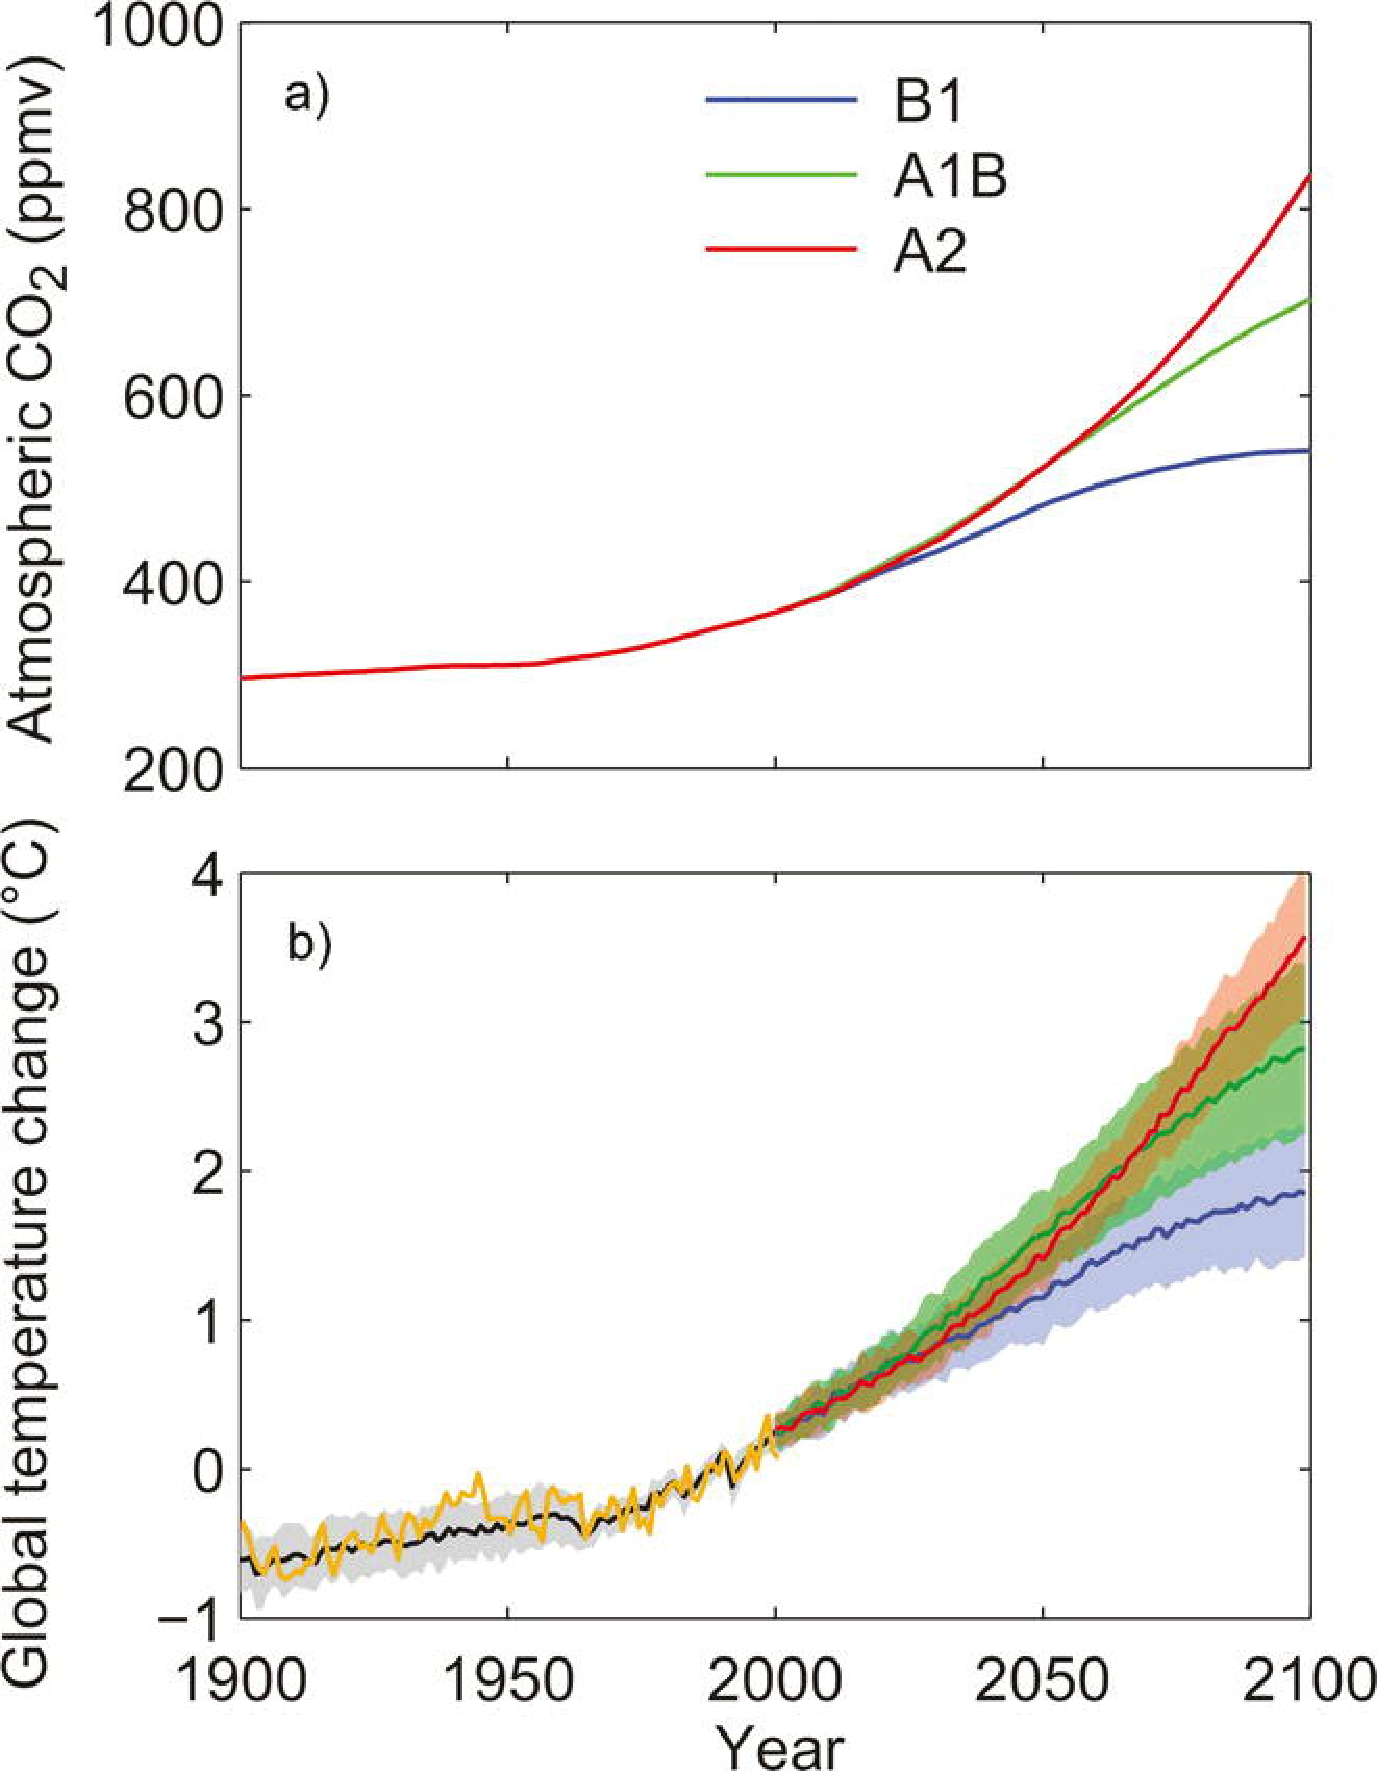
\includegraphics[width=19pc]{figure01.pdf}}
  \caption{Enter the caption for your figure here.  Repeat as
  necessary for each of your figures.}\label{f1}
\end{figure}

\begin{figure}

{\centering 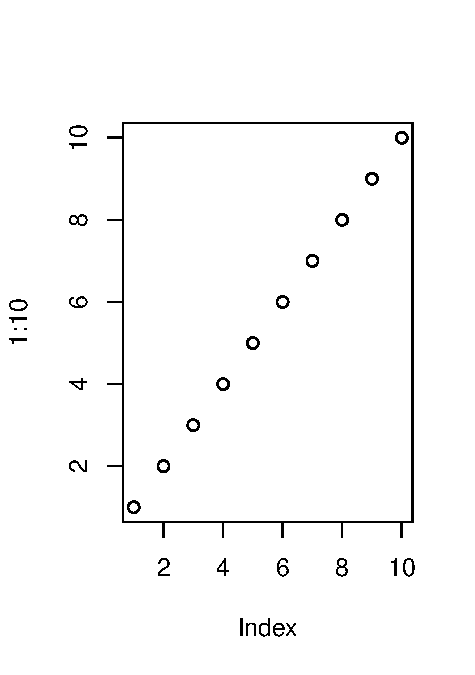
\includegraphics{AMS_files/figure-latex/unnamed-chunk-1-1} 

}

\caption{test the rmd output}\label{fig:unnamed-chunk-1}
\end{figure}

\hypertarget{tables}{%
\subsubsection{Tables}\label{tables}}

Each table must be numbered, provided with a caption, and mentioned
specifically in the text. See below (in the .tex document) and at the
end of the document for the formatting of a sample table (Table
\ref{t1}).

\begin{table}[h]
\caption{This is a sample table caption and table layout.}\label{t1}
\begin{center}
\begin{tabular}{ccccrrcrc}
\topline
$N$ & $X$ & $Y$ & $Z$\\
\midline
 0000 & 0000 & 0010 & 0000 \\
 0005 & 0004 & 0012 & 0000 \\
 0010 & 0009 & 0020 & 0000 \\
 0015 & 0016 & 0036 & 0002 \\
 0020 & 0030 & 0066 & 0007 \\
 0025 & 0054 & 0115 & 0024 \\
\botline
\end{tabular}
\end{center}
\end{table}

\acknowledgments

Keep acknowledgments (note correct spelling: no e between the g and m)
as brief as possible. In general, acknowledge only direct help in
writing or research. Financial support (e.g., grant numbers) for the
work done, for an author, or for the laboratory where the work was
performed is best acknowledged here rather than as footnotes to the
title or to an author's name. Contribution numbers (if the work has been
published by the author's institution or organization) should be
included as footnotes on the title page, not in the acknowledgments.

Please use The authors thank \ldots rather than The authors would like
to thank \ldots.

The author thanks Mats Dahlgren for version one of \textsf{achemso}, and
Donald Arseneau for the code taken from \textsf{cite} to move citations
after punctuation. Many users have provided feedback on the class, which
is reflected in all of the different demonstrations shown in this
document.

\appendix[A]

\appendixtitle{Title of Appendix}

\hypertarget{appendix-section}{%
\subsection{Appendix section}\label{appendix-section}}

The AMS template allows authors to format an unlimited number of
appendixes. To format a single appendix, use the
\texttt{\textbackslash{}appendix} command with no additional argument.
Otherwise, add the appropriate one-letter argument to the
\texttt{\textbackslash{}appendix} command
(e.g.~\texttt{\textbackslash{}appendix{[}A{]}},
\texttt{\textbackslash{}appendix{[}B{]}},
\texttt{\textbackslash{}appendix{[}C{]}}, etc.) corresponding to the
appropriate appendix.

The title of the appendix can be formatted using the
\texttt{\textbackslash{}appendixtitle\{\}} command. The \texttt{\#\#} ,
\texttt{\#\#\#} and \texttt{\textbackslash{}paragraph} commands are used
to create sections within the appendix. (Note that the appendix title
takes the place of \texttt{\#} in the appendix, so the first section
should begin with \texttt{\#\#} instead of \texttt{\#}.)

Equations are automatically numbered appropriately for each appendix.
Here is an example of the first equation in appendix A, automatically
labeled (\ref{eq:1}):

\begin{equation}
\label{eq:1}
x=\frac{2b\pm\sqrt{b^{2}-4ac}}{2c}.  
\end{equation}

For appendix figures and tables, special commands are needed to manually
change the numbering to ensure that each appendix figure or table is
numbered as part of the appendix and not as a continuation of the main
paper. Use the command \texttt{\textbackslash{}appendcaption\{\}}
instead of the usual \texttt{\textbackslash{}caption\{\}} to adjust the
numbering; for example, for Table A1, you would use the command
\texttt{\textbackslash{}appendcaption\{A1\}}. In-text callouts for each
appendix figure and table will need to be written as plain text;the
usual \texttt{\textbackslash{}ref\{\}} command cannot be used.

\appendix[B]
\appendixtitle{File Structure of the AMS \LaTeX\ Package}

\hypertarget{ams-files}{%
\subsection{\texorpdfstring{AMS
\LaTeX~files}{AMS ~files}}\label{ams-files}}

You will be provided with a tarred, zipped \LaTeX~package containing 3
files. These files are

\begin{description}

\item
  your-paper-name.Rmd template for your paper
\item
  amstest.bib an example of a bibliographic database file.
\item
  figure01.pdf are sample figures.

\end{description}

\hypertarget{help-for-authors}{%
\subsection{Help for Authors}\label{help-for-authors}}

Questions and feedback concerning the use of the AMS \LaTeX~files should
be directed to latex@ametsoc.org or yufreecas@gmail.com(for rmarkdown
issues). Additional information is available on the AMS
\LaTeX~Submission Info web page
(\url{http://www2.ametsoc.org/ams/index.cfm/publications/authors/journal-and-bams-authors/author-resources/latex-author-info/}).

\appendix[C]
\appendixtitle{Building a PDF and Submitting Your \LaTeX\ Manuscript Files to the AMS}

\hypertarget{building-your-own-pdf}{%
\subsection{Building your own PDF}\label{building-your-own-pdf}}

There are a variety of different methods and programs that will create a
final PDF from your \LaTeX~files. The easiest method is to download one
of the freely available text editors/compilers such as Rstudio to
compile your files into a PDF.

\hypertarget{submitting-your-files-to-the-ams-for-peer-review}{%
\subsection{Submitting your files to the AMS for peer
review}\label{submitting-your-files-to-the-ams-for-peer-review}}

The AMS uses the Editorial Manager system for all author submissions for
peer review. Editorial Manager uses the freely available \TeX~Live 2011
distribution. This system will automatically generate a PDF from your
submitted \LaTeX~files and figures(not Rmd file, tex files will be
produced when you successful knit your Rmd file).

You should not upload your own PDF into the system. If the system does
not build the PDF from your files correctly, refer to the AMS \LaTeX~FAQ
page first for possible solutions. If your PDF still does not build
correctly after trying the solutions on the FAQ page, email
latex@ametsoc.org for help.

\hypertarget{other-software}{%
\subsection{Other software}\label{other-software}}

As mentioned above, there is a variety of software that can be used to
edit .tex files and build a PDF. The AMS does not support
\LaTeX/-related WYSIWYG software, such as Scientific Workplace, or
WYSIWYM software, such as LyX. \TeX~Live (available online at
\textbackslash{} \url{http://www.tug.org/texlive/}) is recommended for
users needing an up-to-date \LaTeX~distribution with software that
includes an editor and the ability to automatically generate a PDF.

\hypertarget{references}{%
\section*{References}\label{references}}
\addcontentsline{toc}{section}{References}

\bibliography{references}

\begin{table}
\appendcaption{A1}{Here is the appendix table caption.}
\centering
\begin{tabular}{ccc}
\topline
$1$ & $2$ & $3$ \\
\midline
a&b&c \\
d&e&f \\
\botline
\end{tabular}
\end{table}

\begin{figure}
\centerline{(illustration here)}
\appendcaption{A1}{Here is the appendix figure caption.}
\end{figure}

\begin{figure}
\centerline{(illustration here)}
\appendcaption{B1}{Here is the appendix figure caption.}
\end{figure}

\hypertarget{refs}{}
\leavevmode\hypertarget{ref-alexander:2002}{}%
Alexander, M. A., I. Bladé, M. Newman, J. R. Lanzante, N.-C. Lau, and J.
D. Scott, 2002: The atmospheric bridge: The influence of ENSO
teleconnections on air--sea interaction over the global oceans. \emph{J.
Climate}, \textbf{15}, 2205--2231,
doi:\href{https://doi.org/10.1175/1520-0442(2002)015\%3C2205:tabtio\%3E2.0.co;2}{10.1175/1520-0442(2002)015\textless2205:tabtio\textgreater2.0.co;2}.

\leavevmode\hypertarget{ref-Gershunov2012}{}%
Gershunov, A., and K. Guirguis, 2012: California heat waves in the
present and future. \emph{Geophys.~Res.~Lett.}, \textbf{39},
doi:\href{https://doi.org/10.1029/2012GL052979}{10.1029/2012GL052979}.

\leavevmode\hypertarget{ref-poe12}{}%
Pöhlker, C. and Coauthors, 2012: Biogenic potassium salt particles as
seeds for secondary organic aerosol in the Amazon. \emph{Science},
\textbf{337}, 1075--1078.
\end{document}
